\chapter{基于多尺度网络结构的故障诊断模型研究}

\section{引言}

在第~\ref{cha:chapter3}章中,我们设计了一个结构与VGG类似的卷积神经网络模型来完成故障
模式的学习和预测。从该模型的结构示意图~\ref{fig:cnn_classifier}以及各层特征图的数据维
度变化图~\ref{fig:cnn_data}可以看出,在网络中的特征提取阶段,由于下采样层的存在,网络
每经过一个图~\ref{fig:cnn_classifier}中虚线框表示的基本单元,特征图在空间的尺寸就会减
半。我们知道,下采样层的作用是从输入数据中筛选出显著特征,因此经过多个下采样层之后,
输入数据的整体特征被提取出来,而局部特征被丢弃。这一点从~\ref{subsection:cascade_result}
节给出的实验结果也可以得到印证。在~\ref{subsection:cascade_result}中我们比较了不同核
宽度的平均值下采样提取的特征向量,这里我们将核宽度$F$分别等于2、4、8、16、32时,使用单
层平均值下采样提取的特征向量绘制成图~\ref{fig:features_scales}。可以看出,下采样程度
越大,提取的特征中保留的原始信号频谱序列的细节信息就越少。
\begin{figure}[ht]
  \centering
  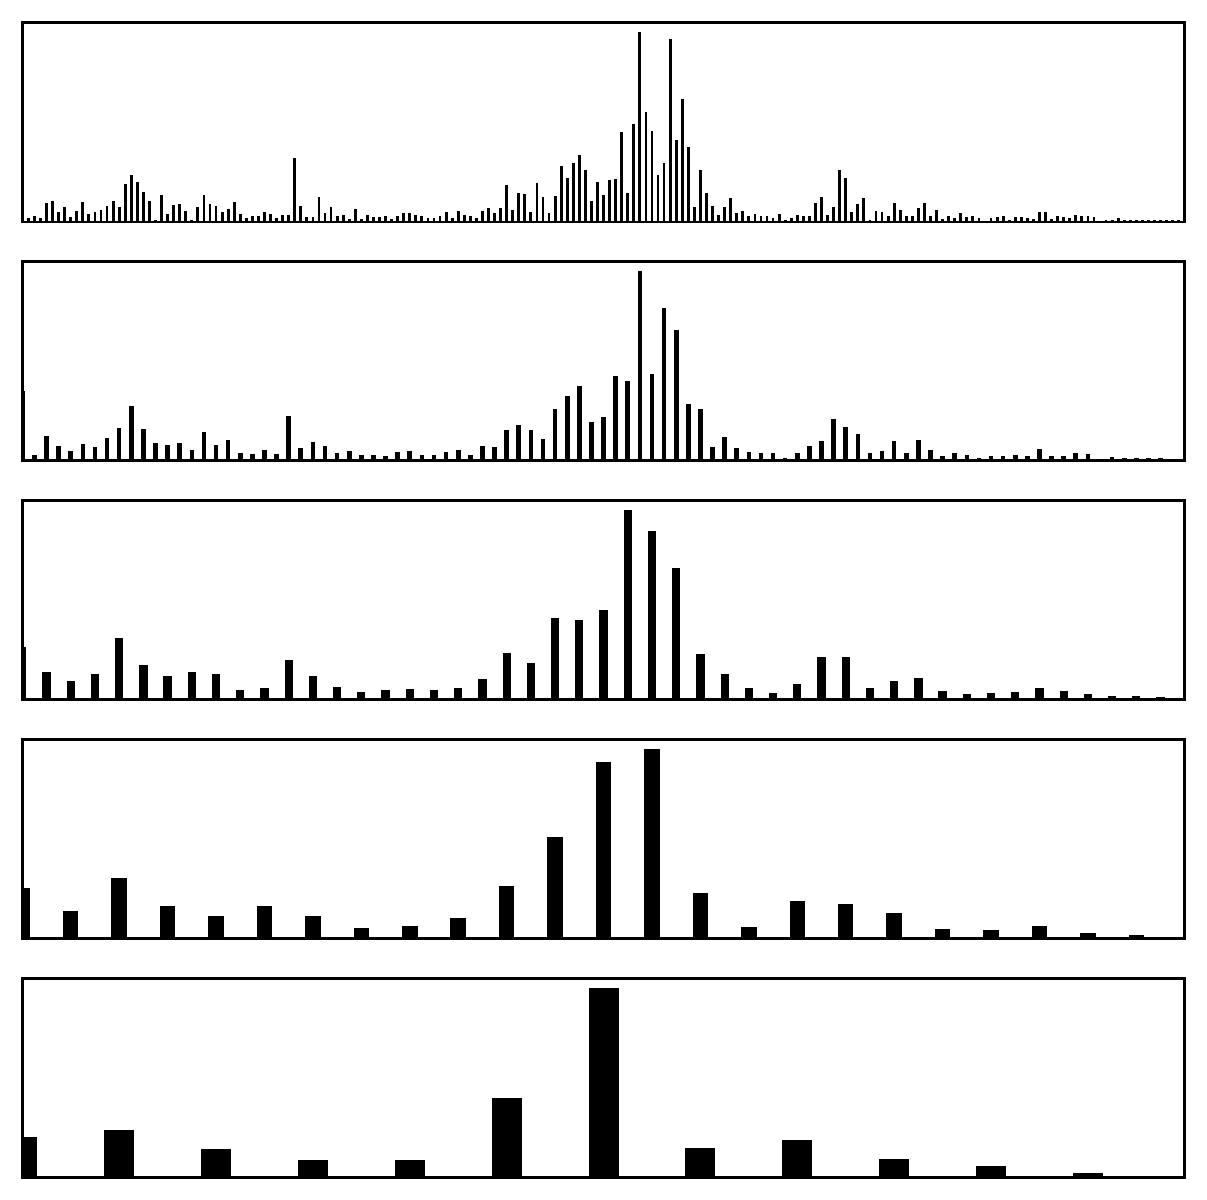
\includegraphics[height=10cm]{features_scales}
  \caption{不同采样程度下提取的特征向量}
  \label{fig:features_scales}
\end{figure}

总体上讲,这样的特征提取过程有助于分析输入数据和输出标签之间的联系,但是如果这些局部
特征在特征提取的过程中能够在一定程度上得到保留,或者是跟下采样得到的整体特征加以融合,
那么一定能够提升模型对输入数据的理解程度,从而提升模型最终的预测精度。

本章首先介绍了一个新的网络层——上采样(Upsampling)层。然后设计了一个递归的网络结构,
使得模型在特征提取阶段能够将经过下采样之后的整体特征和下采样前的局部特征进行融合,从
而使得模型最终提取的特征向量中也包含输入数据的细节信息。最后使用该模型在CWRU数据集上
进行仿真实验,得到了比第~\ref{cha:chapter2}章和第~\ref{cha:chapter3}章都要更好的预测
精度。此外,本章还将实验中获得的结果与其他论文在该数据集上获得的效果进行了对比。

\section{上采样}

在~\ref{subsection:cnn}节中,我们介绍了卷积神经网络中经常使用的下采样层,输入数据在
经过下采样层之后空间的尺寸会减小。例如图片经过下采样之后图片的宽度和高度会减小,得到
分辨率更低的缩略图。我们也可以通过上采样操作向图片中添加像素,从而增大图片的尺寸。

上采样的过程实际上是通过插值算法来完成的,下面我们对使用最近邻插值算法进行上采样的
过程做简单介绍。例如我们要将原始图像放大3倍,那么图像中原本的像素位置随着图像尺寸的
变大而向外扩张,因此各行(列)像素间将会产生空隙,根据最近邻插值算法,我们可以使用离
得最近的像素值来填补这些空隙。也就是将原始图像中的每个像素值沿宽度和高度方向均重复3
次,变成$3\times 3$个像素。如图~\ref{fig:nn_upsampling}所示。
\begin{figure}[ht]
  \centering
  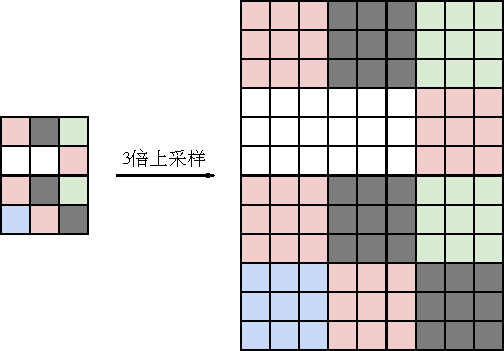
\includegraphics{nn_upsampling}
  \caption{最近邻插值算法示意图}
  \label{fig:nn_upsampling}
\end{figure}

除最近邻插值算法外,常见的还有双线性插值算法、双三次插值算法等。还有一些针对特定放大
比例的算法,例如在放大2倍、3倍或4倍时分别对应的hq2x、hq3x和hq4x算法等。图
~\ref{fig:image_upsampling}是不同插值算法在同一张图片上实现的上采样结果示例。
\begin{figure}[ht]
  \centering
  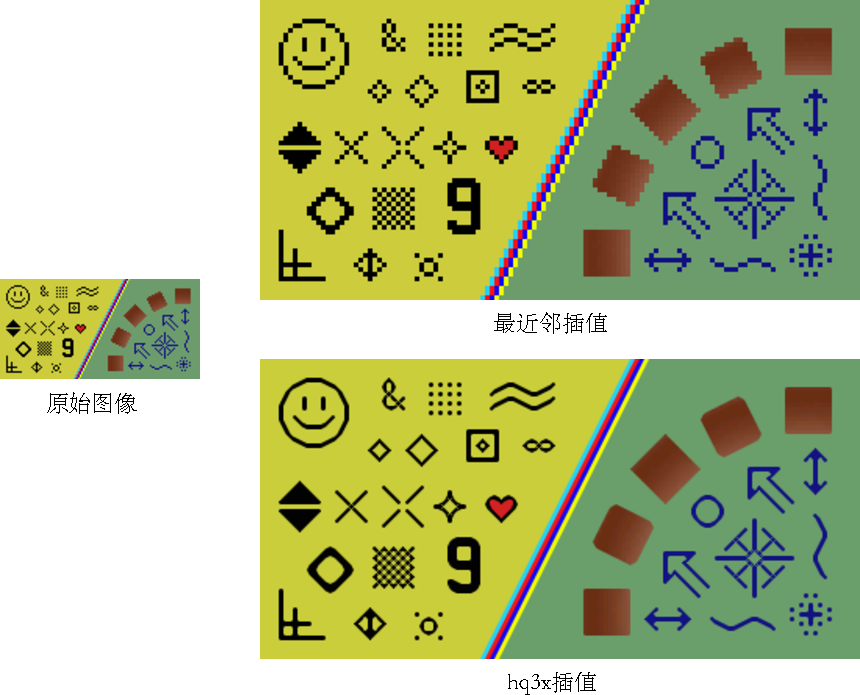
\includegraphics[width=12cm]{image_upsampling}
  \caption{两种插值算法在同一张图片上的上采样结果示例}
  \label{fig:image_upsampling}
\end{figure}

在卷积神经网络中,同下采样层一样,上采样层也是独立操作特征图深度方向上的每一个切片,
用指定的插值算法来对每个切片在空间上的尺寸进行放大。上采样层同样也不改变特征图的深度,
并且也不会向网络中引入参数。一般地,如果上采样层输入的特征图维度为
$W_1\times H_1\times D_1$,放大比例为$S$,输出的特征图维度为$W_2\times H_2\times D_2$,
那么有:
\begin{equation}
  \label{equ:chap4:upsampling_dim}
  \left\{\begin{aligned}
    & W_2 = W_1 \cdot S \\
    & H_2 = H_1 \cdot S \\
    & D_2 = D_1
  \end{aligned}\right.
\end{equation}

\section{基于多尺度网络结构的故障诊断模型}

\begin{figure}[ht]
  \centering
  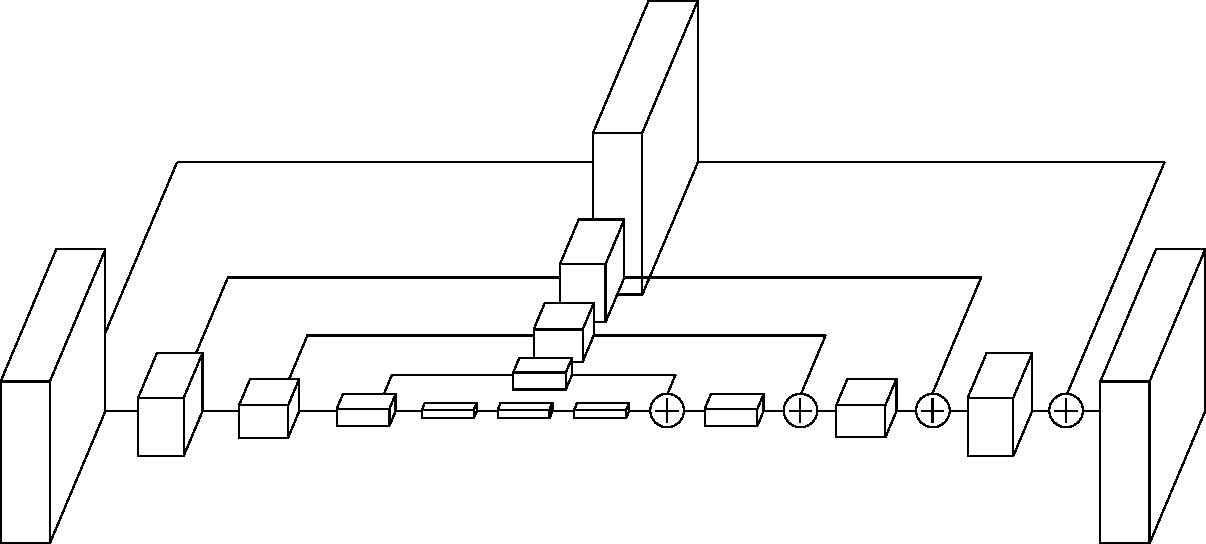
\includegraphics[width=14cm]{cnn_ms}
  \caption{多尺度网络结构的故障诊断模型}
  \label{fig:cnn_ms}
\end{figure}

\section{仿真实验}

\subsection{实验过程}

\subsection{实验结果及分析}

\section{小结}
